% !TEX root = ../thesis-example.tex
%
\chapter*{Introduction Générale}
\label{chap:intro}
\addcontentsline{toc}{chapter}{\nameref{chap:intro}}

\section{Contexte et Motivations}
\label{sec:intro:contexte}
Une décision judiciaire peut être définie soit comme  le résultat rendu par des juges à l'issue d'un procès, ou bien un document décrivant une affaire judiciaire en résumant les faits, les procédures suivies, la solution des juges, et les raisons qui les y ont conduits. %Nous considérons le nom "résultat" pour la première définition, et pour la seconde, "décision jurisprudentielle", "décision judiciaire", "décision de justice" ou simplement  "décision".
Les décisions judiciaires sont essentielles pour les juristes parce qu'elles sont des sources d'interprétation de la loi. Les juristes ont l'habitude d'en collecter, sélectionner et analyser pour résoudre les problèmes auxquels ils s'intéressent afin de mieux comprendre \citep{ancel2003expulsion} et anticiper (par ex. les avocats pour leur clients) les décisions des juges. Généralement manuelle, cette analyse rencontre quelques limites. D'abord, l'accès à un corpus exhaustif de décisions est difficile vu l'énorme volume de décisions réparti dans les juridictions (plus de 4 millions de décisions en France par an d'après les chiffres du ministère français de la justice \footnote{\url{http://www.justice.gouv.fr/budget-et-statistiques-10054/chiffres-cles-de-la-justice-10303/}} comme l'illustre le Tableau \ref{tab:intro:nbdecisionstats}). Malgré la disponibilité d'un nombre important de décisions en ligne, les moteurs de recherche juridiques proposent essentiellement des critères à mots-clés. 
\begin{table}[!h]
{
\scriptsize
\begin{center}
\begin{tabular}{|p{2cm}|c|c|c|c|c|}
\hline
 & \textbf{2010} & \textbf{2011} & \textbf{2012} & \textbf{2013} & \textbf{2014} \\
 \hline
 \textbf{Justice civile} & 2 673 131  & 2 654 179 & 2 647 813 & 2 761 554  & 2 618 374 \\
 \hline
Justice pénale & 1 173 242 & 1 180 586 & 1 251 979 & 1 303 469 & 1 203 339 \\
 \hline
 Justice administrative & 224 787 & 225 608 & 228 680 & 221 882 & 230 477 \\
 \hline
\end{tabular}

\textit{\scriptsize{Source: \url{http://www.justice.gouv.fr/budget-et-statistiques-10054/chiffres-cles-de-la-justice-10303/}}}  
\end{center}
}
\caption{Nombre de décisions prononcées en France par an}\label{tab:intro:nbdecisionstats}
\end{table}

D'autre part, l'analyse manuelle de décisions peut devenir pénible lorsque les documents sont longs et nombreux.  Par ailleurs, la justice est complexe et son langage difficilement compréhensible \citep{cretin2014justicecomplexe} pour permettre aux non-juristes d'estimer le risque judiciaire qu'ils encourent sans l'aide d'un initié en droit. D'une part, une analyse automatisée des décisions jurisprudentielles peut aider des avocats et chercheurs en droit à comprendre l'opinion des juges sur certaines questions. D'autre part, elle constitue potentiellement une aide précieuse pour les particuliers et entreprises soucieux de connaitre les chances que leurs requêtes aboutissent en justice.  De telles analyses sont indispensables pour les pratiquants du droit car elles fournissent un ensemble important d'information d'une valeur inestimable dont notamment un aperçu de l'application de la loi. L'extraction automatique d'information pertinente à cette étude aiderait à mieux décrire et organiser les décisions tout en enrichissant les critères de recherche avec par exemple les noms de juges ou les articles de loi. Ce mémoire présente les résultats d'une étude visant à automatiser l'extraction d'information à partir de ces documents afin de faciliter la recherche et les analyses descriptives et prédictives d'un corpus jurisprudentiel. La principale motivation est l'exhaustivité qui passe nécessairement par un traitement rapide et efficace de la grande masse de documents produit par la justice. La question à la base de notre étude est celle de savoir "Comment exploiter un corpus de décisions pour analyser, voire prédire, les décisions des juges sachant que l'interprétation subjective des règles juridiques rend l'application de la loi non déterministe ?". Cette question intéresse de nombreuses entreprises telles que LexisNexis avec son système LexMachina\footnote{\url{https://lexmachina.com}}, et de jeunes startups françaises telles que Predictice\footnote{\url{http://predictice.com}} et CASE LAW ANALYTICS\footnote{\url{http://caselawanalytics.com}}. Afin d'y répondre, nous sommes partis d'une conception théorique considérant la demande ou prétention des parties comme le concept central d'une décision (Figure \ref{fig:intro:demande-central}) et tout autour s'affectent d'autres concepts, notamment, le résultat des juges relatif à cette prétention, le fondement juridique de la prétention ou norme, la catégorisation des prétentions, et ensuite les différentes circonstances factuelles dans lesquelles cette prétention est généralement formulée. 

\begin{figure}[h]
    \centering
    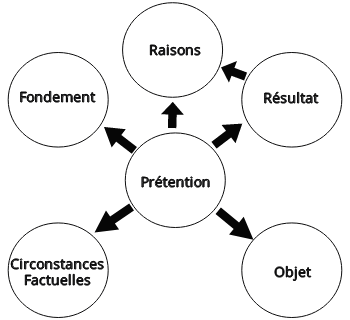
\includegraphics[scale=0.75]{demande-central.png}
    \caption{La demande est centrale aux concepts liés à l'analyse des décisions}
    \label{fig:intro:demande-central}
\end{figure}

En fait, La granularité de l'analyse est affinée jusqu'à la demande car dans une décision, les juges apportent une réponse à chaque demande, et par conséquent une partie peut voir certaines de ses demandes acceptées complètement, lorsque d'autres accordées partiellement, et le reste est rejetée.  Ceci revoit en effet les modélisations prédictives qui ne s'attardaient qu'à déterminer globalement si le plaintif a  gagné ou perdu le procès sans estimer précisement ce que chaque partie a obtenu. Un juriste sera donc plus intéressé à formuler les demandes qui ont de meilleures chances d'être acceptées qu'à prévoir une victoire du procès. Par ailleurs, les juristes s'intéressent généralement à un type de contentieux à la fois et surtout à des types particuliers de demandes s'appuyant sur une règle ou un principe juridique appelé "fondement". Ainsi, une analyse devrait se faire dans un contexte bien précis, défini par ces différents concepts.


\section{Enoncé des problèmes}
\label{sec:intro:probleme}
L'analyse automatique de décisions jurisprudentielles fait références à de nombreux problèmes rencontrés par les juriste lors de leur analyse manuelle (\textcolor{red}{par exemple?}). Dans le cadre de notre travail, nous avons définies et traités les quelques problèmes principaux décrits dans les sous-sections suivantes.
\subsection{Sectionnement des documents}
Le sectionnement des décisions de justice est important pour donner une première structure grossière aux documents. Cette structuration pourrait faciliter tout autant la lecture manuelle des documents par la localisation plus rapide des informations, et l'organisation des tâches d'extraction automatique d'information. Notre principale contribution lors du traitement de ce problème a été de réaliser une étude comparative de modèles d'étiquetage de séquence, bien établis au sein de la communauté de traitement automatique du langage naturel (TALN),  pour la reconnaissance de sections prédéfinies. 

\subsection{Annotation de métadonnées}

\subsection{Identification de données relatives aux demandes}

\subsection{Identification des circonstances factuelles}

\section{Méthodologie}
\label{sec:intro:methodologie}


\section{Résultats}
\label{sec:intro:résultats}

\section{Structure du mémoire}
\label{sec:intro:organisation}

\textbf{Chapitre \ref{sec:literature}} \\[0.2em]
%blindtext

\textbf{Chapitre \ref{sec:structuration}} \\[0.2em]
%\blindtext

\textbf{Chapitre \ref{sec:quanta}} \\[0.2em]
%\blindtext

\textbf{Chapitre \ref{sec:sensresultat}} \\[0.2em]
%\blindtext

\textbf{Chapitre \ref{sec:similarite}} \\[0.2em]
%\blindtext

\textbf{Chapitre \ref{sec:conclusion}} \\[0.2em]

\textbf{Les annexes \ref{sec:demo}} \\[0.2em]
